\documentclass[micros_g1_main.tex]{subfiles}
\begin{document}

\section{}

Se estudi\'o el comportamiento del microprocesador HC11 al correr el siguiente programa:

	\begin{lstlisting}
	org	$2000
	ldaa	$C000
	jmp	$2000
	\end{lstlisting}

En primer lugar, se realiz\'o un an\'alisis te\'orico de lo que esperaba verse. El mismo se encuentra plasmado en la figura \ref{fig:teorico}. Luego, se procedi\'o a observar estas se\~nales en el osciloscopio.

\begin{figure}[ht]
	\centering
	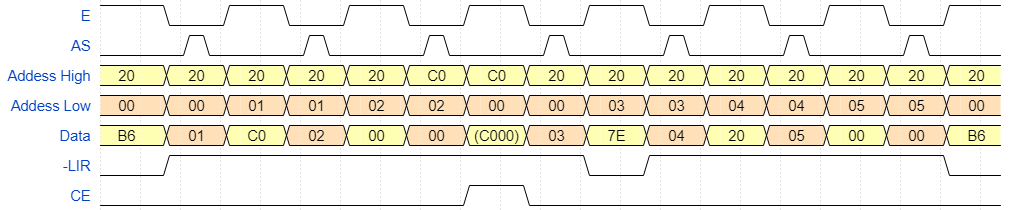
\includegraphics[width=\textwidth]{images/micros-g1-waves.png}
	\caption{Diagrama de tiempos del programa analizado}
	\label{fig:teorico}
\end{figure}

\begin{figure}[ht]
	\centering
	\fbox{
	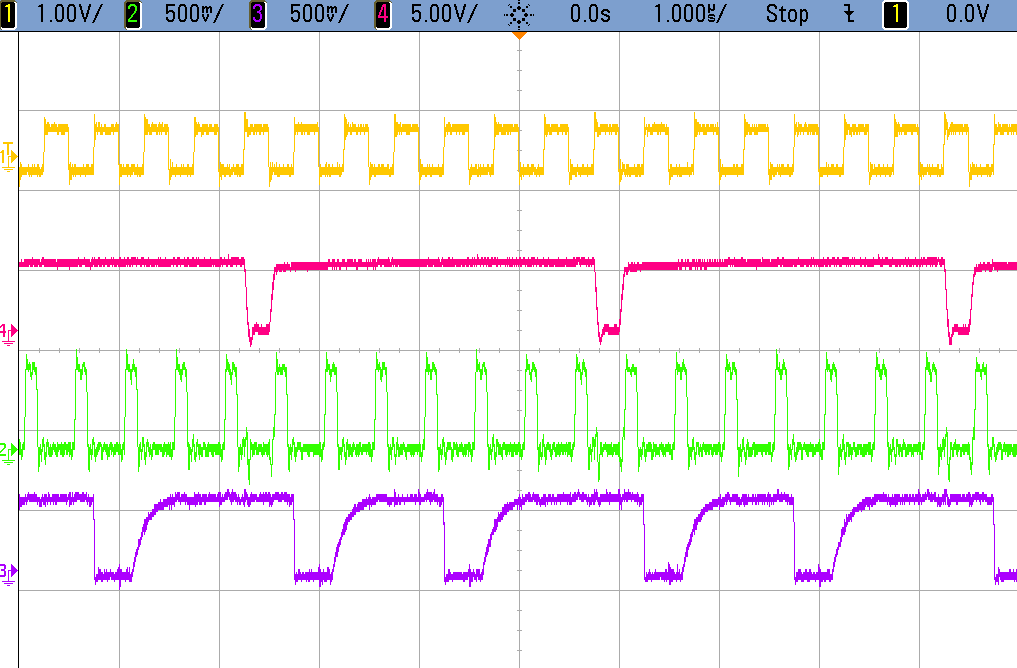
\includegraphics[width=0.8\textwidth]{images/micros-g1-ej1-1.png}
	}
	\caption{Medici\'on de E (amarillo), $\overline{\text{CE}}$ de la flash (rosa), AS (verde), y $\overline{\text{LIR}}$ (violeta)}
\end{figure}


A grandes rasgos, el comportamiento observado coincide con el esperado. Se observa que las transiciones en el LIR son mucho m\'as lentas que en las dem\'as se\~nales, y es a su vez la \'unica que no presenta sobrepicos. Esta se\~nal nos permite saber qu\'e instrucci\'on se est\'a ejecutando: cuando el tiempo entre dos pulsos activos (bajos) es m\'as largo, se est\a corriendo "ldaa C000", y cuando es m\'as corto, "jmp 2000". 

Por otro lado, el chip select nos permite identificar el momento en que se accede a la posici\'on C000, que es la \'unica de las que utiliza el programa que se encuentra en la memoria flash. En la figura \ref{fig:chip-enable}, se observa que cuando E est\'a en 0, ninguno de los chips est\'a seleccionado. Cuando est\'a en 1, el chip select de la RAM pasa a activo (bajo), salvo cuando se accede a la posici\'on C000.

\begin{figure}[ht]
	\centering
	\fbox{
	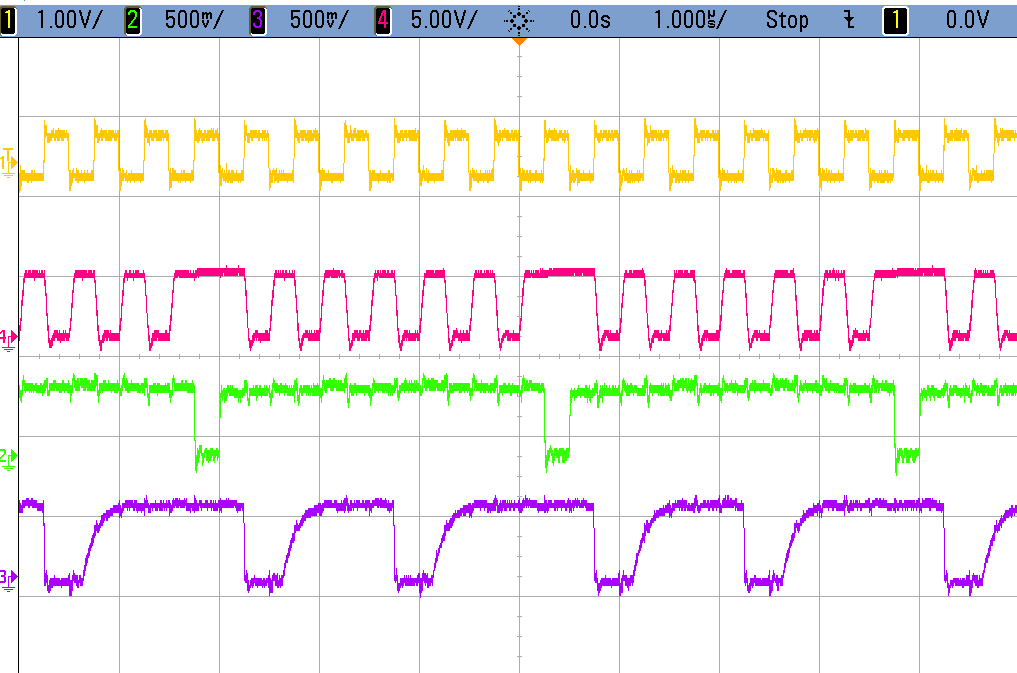
\includegraphics[width=0.8\textwidth]{images/micros-g1-ej1-2.png}
	}
	\caption{Medici\'on de E (amarillo), $\overline{\text{CE}}$ de la RAM (rosa), $\overline{\text{CE}}$ de la flash (verde), y $\overline{\text{LIR}}$ (violeta)}
	\label{fig:chip-enable}
\end{figure}

En cuanto a los buses, se observaron algunas se\~nales y se verific\'o que las mismas tomaban los valores de la figura \ref{fig:teorico}. A modo ilustrativo, se incluyen mediciones de los bits 14 y 15 del bus de direcciones en la figura \ref{fig:address-bus}. Como las instrucciones que se ejecutan en este programa est\'an entre las direcciones 2000 y 2005, la parte alta del bus de address es siempre 20, salvo cuando se accede a la posici\'on C000. Por lo tanto, cuando el nybble m\'as significativo pasa de 2 (0010) a C (1100), los bits 14 y 15 se inviterten.

\begin{figure}[ht]
	\centering
	\fbox{
	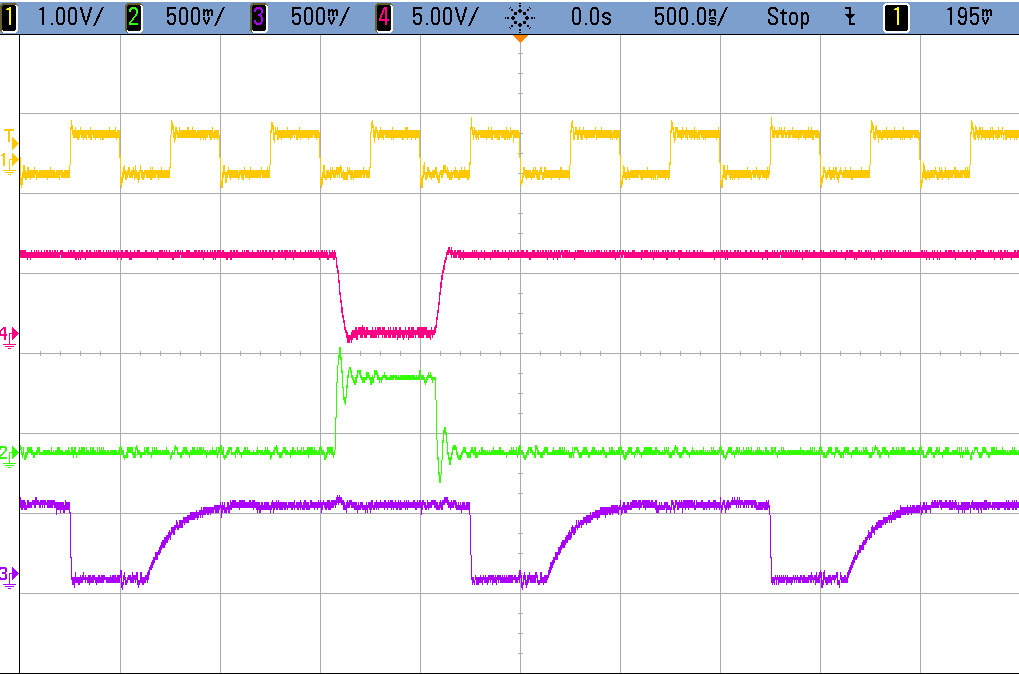
\includegraphics[width=0.8\textwidth]{images/micros-g1-ej1-3.png}
	}
	\caption{Medici\'on de E (amarillo), A14(rosa), A15 (verde), y $\overline{\text{LIR}}$ (violeta)}
	\label{fig:address-bus}
\end{figure}


\end{document}
